\newgeometry{top=2cm,left=2cm,right=2cm,bottom=2cm} 
%
\section{Derivation of the BTZ metric}
As we proved in the last section, all vacuum solutions to the \textbf{Einstein Equations} in (2+1) dimensions are locally isomorphic to either de Sitter space, anti-de Sitter space or Minkowski space. Thus, all the information about any particular solution will be contained in its topology. Despite this, it is still very worthwhile to derive the BTZ metric in what we will call \textbf{Schwarzschild-like coordinates}, under the assumptions of stationarity and circular symmetry. There are several reasons for this, some of which being: it is easy to identify event horizons, the mass and angular momentum parameters will stand out clearly and the description of the spacetime in terms of identifying points in $AdS_3$ will be particularly simple. With all that said, let us begin the derivation.

\subsection{An ansatz for the Einstein Equations}
On a $3$-dimensional spacetime, a general metric tensor will have $3 \, (3 + 1) / 2 = 6$ independent components, $3$ of which can be arbitrarily changed by coordinate transformations. We will use this freedom to assume the following form of the metric: 
%
%
\begin{equation}\label{2.1}
ds^2 = -f^2(t,r,\phi) \, \mathrm{d}t^2
+ g^2(t,r,\phi) \, \mathrm{d}r^2
+ r^2 \, [\mathrm{d}\phi - h(t,r,\phi) \, \mathrm{d}t]^2
\end{equation}
%
%
We will discuss the ranges of these coordinates when the metric is fully derived. We assume of (\ref{2.1}) that it be both stationary and circularly symmetric. This corresponds to the metric possessing two \textbf{Killing vectors}: $R = \partial_{\phi}$, $K = \partial_t$. In order for (\ref{2.1}) to be invariant under the flow of $R$ and $K$, the metric must satisfy the conditions:
%
%
\begin{align}\label{2.2}
\mathcal{L}_{R} \, g_{\mu \nu} & =
R^{\lambda} \, \frac{\partial g_{\mu \nu}}{\partial x^{\lambda}}
+ g_{\lambda \nu} \, \frac{\partial R^{\lambda}}{\partial x^{\mu}}
+ g_{\mu \lambda} \, \frac{\partial R^{\lambda}}{\partial x^{\nu}} =
\frac{\partial g_{\mu \nu}}{\partial \phi} = 0
\notag\\
\mathcal{L}_{K} \, g_{\mu \nu} & =
K^{\lambda} \, \frac{\partial g_{\mu \nu}}{\partial x^{\lambda}}
+ g_{\lambda \nu} \, \frac{\partial K^{\lambda}}{\partial x^{\mu}}
+ g_{\mu \lambda} \, \frac{\partial K^{\lambda}}{\partial x^{\nu}} =
\frac{\partial g_{\mu \nu}}{\partial t} = 0
\end{align}
%
%
Where $\mathcal{L}_{X}$ is the \textbf{Lie derivative} in the direction of the vector $X$. The conditions (\ref{2.2}) simply implies that the components of the metric be independent of $\phi$ and $t$. We can thus write the metric (\ref{2.1}), our ansatz for the Einstein Equations, in the form:
%
%
\begin{equation}\label{2.3}
ds^2 = -f^2(r) \, \mathrm{d}t^2
+ g^2(r) \, \mathrm{d}r^2
+ r^2 \, [\mathrm{d}\phi - h(r) \, \mathrm{d}t]^2
\end{equation}
%
%


\subsection{Solving the Einstein Equations}
In section 1.3 on Einstein gravity in (2+1) dimensions, we found that the vacuum \textbf{Einstein equations} on a $3$-dimensional spacetime, could be brought to the following form:
%
%
\begin{equation}\label{2.7}
R_{ij} = 2 \, \Lambda \, g_{ij}
\end{equation}
%
%
In order to find solutions to (\ref{2.7}), we first compute the \textbf{Ricci tensor} $R_{ij}$. We will do this using the \textbf{orthonormal frame method}, also sometimes called the triad method. We start by constructing an orthonormal basis of 1-forms $\epsilon^i$:
%
%
\begin{equation}
\epsilon^0 = f(r) \, \mathrm{d}t
\quad , \quad
\epsilon^1 = g(r) \, \mathrm{d}r
\quad , \quad
\epsilon^2 = r \, [\mathrm{d}\phi
- h(r) \, \mathrm{d}t]
\end{equation}
%
%
In the basis of the orthonormal 1-forms $\epsilon^i$, the metric manifestly becomes diagonal, meaning that:
%
%
\begin{equation}
ds^2 = \eta_{ij} \, \epsilon^i \otimes \epsilon^j
= -\epsilon^0 \otimes \epsilon^0
+ \epsilon^1 \otimes \epsilon^1
+ \epsilon^2 \otimes \epsilon^2
\end{equation}
We can now employ the orthonormal 1-form basis $\epsilon^i$ to find the \textbf{connection 1-forms} ${\omega^i}_j$, using the first \textbf{Cartan structure equation}:
%
%
\begin{equation}\label{2.9}
\Theta^i = \mathrm{d}\epsilon^i + {\omega^i}_j \wedge \epsilon^j = 0
\end{equation}
%
%
The components $g_{ij}$ are the metric components with respect to the basis $\epsilon^i$, and $\Theta^i$ are the \textbf{torsion 2-forms}. The requirement that our connect be torsion-free and metric compatible, impose the following requirements on $\Theta^i$ and ${\omega^i}_j$:
%
%
\begin{equation}\label{reqs}
\Theta^i = 0
\quad , \quad
\omega_{ij} = -\omega_{ji}
\quad , \quad
\omega_{ij} := g_{ik} \, {\omega^k}_j
\end{equation}
%
%
We now look for solutions to (\ref{2.9}) satisfying the requirements (\ref{reqs}). We start by computing the exterior derivative of our basis 1-forms $\epsilon^i$:
\begin{equation}
\mathrm{d}\epsilon^0 = F(r) \, \epsilon^1 \wedge \epsilon^0
\quad , \quad
\mathrm{d}\epsilon^1 = 0
\quad , \quad
\mathrm{d}\epsilon^2 = G(r) \, \epsilon^1 \wedge \epsilon^2
- H(r) \, \epsilon^1 \wedge \epsilon^0
\end{equation}
%
%
Here, the functions $F(r)$, $G(r)$ and $H(r)$, are given in terms of $f(r)$, $g(r)$ and $h(r)$ by:
%
%
\begin{equation}\label{2.11}
F(r) := \frac{f'(r)}{f(r) \, g(r)}
\quad , \quad
G(r) := \frac{1}{r \, g(r)}
\quad , \quad
H(r) := \frac{r \, h'(r)}{f(r) \, g(r)}
\end{equation}
%
%
The structure equation (\ref{2.9}) with restrictions (\ref{reqs}) in our orthonormal basis $\epsilon^i$ then becomes:
%
%
\begin{align}
F(r) \, \epsilon^1 \wedge \epsilon^0
+ {\omega^0}_1 \wedge \epsilon^1
+ {\omega^0}_2 \wedge \epsilon^2 & = 0
\notag\\
{\omega^1}_0 \wedge \epsilon^0
+ {\omega^1}_2 \wedge \epsilon^2 & = 0
\notag\\
G(r) \, \epsilon^1 \wedge \epsilon^2
- H(r) \, \epsilon^1 \wedge \epsilon^0
+ {\omega^2}_0 \wedge \epsilon^0
+ {\omega^2}_1 \wedge \epsilon^1 & = 0
\end{align}
%
Upon inspection, one finds that the following is a set of solutions to the above equations:
%
%
\begin{equation}
{\omega^0}_1 = F(r) \, \epsilon^0 - \frac{1}{2} \, H(r) \, \epsilon^2
\quad , \quad
{\omega^2}_1 = G(r) \, \epsilon^2 - \frac{1}{2} \, H(r) \, \epsilon^0
\quad , \quad
{\omega^2}_0 = \frac{1}{2} \, H(r) \, \epsilon^1
\end{equation}
%
%
We can now use the second \textbf{Cartan structure equation} to compute the \textbf{curvature 2-forms}:
%
%
\begin{equation}\label{2.10}
{\Omega^i}_j = \mathrm{d}{\omega^i}_j + {\omega^i}_k \wedge {\omega^k}_j
\end{equation}
%
%
We begin by computing the exterior derivative of each connection 1-form. The result is the following:
%
%
\begin{align}
\mathrm{d}{\omega^0}_1 & = \bigg[ \frac{F'(r)}{g(r)}
+ F^2(r)
- \frac{H^2(r)}{2} \bigg] \, \epsilon^1 \wedge \epsilon^0
%
+ \bigg[ \frac{H'(r)}{2 \, g(r)}
+ \frac{H(r) \, G(r)}{2} \bigg] \, \epsilon^1 \wedge \epsilon^2
\notag\\
\mathrm{d}{\omega^2}_1 & = \bigg[ \frac{G'(r)}{g(r)}
+ G^2(r) \bigg] \, \epsilon^1 \wedge \epsilon^2
%
- \bigg[ G(r) \, H(r)
+ \frac{H'(r)}{2 \, g(r)}
+ \frac{H(r) \, F(r)}{2} \bigg] \, \epsilon^1 \wedge \epsilon^0
\notag\\
\mathrm{d}{\omega^2}_0 & = 0
\end{align}
%
%
We now compute the wedge products between the connection 1-forms. The result is the following:
%
%
\begin{align}\label{struct_2_1}
{\omega^0}_2 \wedge {\omega^2}_1 & = \frac{H(r) \, G(r)}{2} \, \epsilon^1 \wedge \epsilon^2
- \frac{H^2(r)}{4} \, \epsilon^1 \wedge \epsilon^0
\notag\\
{\omega^2}_0 \wedge {\omega^0}_1 & = \frac{H(r) \, F(r)}{2} \, \epsilon^1 \wedge \epsilon^0
+ \frac{H^2(r)}{4} \, \epsilon^1 \wedge \epsilon^2
\notag\\
{\omega^2}_1 \wedge {\omega^1}_0 & = -\bigg[ G(r) \, F(r)
+ \frac{H^2(r)}{4} \bigg] \, \epsilon^0 \wedge \epsilon^2
\end{align}
%
%
Usings the results (\ref{struct_2_1}) and (\ref{struct_2_2}), we see that the second Cartan structure equation (\ref{2.10}) reads:
%
%
\begin{align}\label{struct_2_2}
{\Omega^0}_1 & = \bigg[ \frac{F'(r)}{g(r)}
+ F^2(r)
- \frac{3 \, H^2(r)}{4} \bigg] \, \epsilon^1 \wedge \epsilon^0
%
+ \bigg[ \frac{H'(r)}{2 \, g(r)}
+ H(r) \, G(r) \bigg] \, \epsilon^1 \wedge \epsilon^2
\notag\\
{\Omega^2}_1 & = \bigg[ \frac{G'(r)}{g(r)}
+ G^2(r)
+ \frac{H^2(r)}{4} \bigg] \, \epsilon^1 \wedge \epsilon^2
%
- \bigg[ G(r) \, H(r)
+ \frac{H'(r)}{2 \, g(r)} \bigg] \, \epsilon^1 \wedge \epsilon^0
\notag\\
{\Omega^2}_0 & = -\bigg[ G(r) \, F(r)
+ \frac{H^2(r)}{4} \bigg] \, \epsilon^0 \wedge \epsilon^2
\end{align}
%
%
The curvature 2-forms are related to the \textbf{Riemann tensor} components ${R^i}_{jkl}$, in the following way:
%
%
\begin{equation}
{\Omega^i}_j = \frac{1}{2} \, {R^i}_{jkl} \, \epsilon^k \wedge \epsilon^l
\end{equation}
%
%
The non-zero components (\textit{excluding those related by symmetry}) of the Riemann tensor are thus:
%
%
\begin{align}\label{2.14}
{R^0}_{110} & = \frac{F'(r)}{g(r)} + F^2(r) - \frac{3 \, H^2(r)}{4}
\notag\\
{R^0}_{112} & = \frac{H'(r)}{2 \, g(r)} + H(r) \, G(r)
\notag\\
{R^2}_{112} & = \frac{G'(r)}{g(r)} + G^2(r) + \frac{H^2(r)}{4}
\notag\\
{R^2}_{002} & = -G(r) \, F(r) - \frac{H^2(r)}{4}
\end{align}
%
%
From the above components of the Riemann tensor, we can now construct the non-zero components (\textit{excluding those related by symmetry}) of the \textbf{Ricci tensor} $R_{jl} := {R^i}_{jil}$. The result is the following:
%
%
\begin{align}
R_{00} & = \frac{F'(r)}{g(r)} + F^2(r) - \frac{H^2(r)}{2}
+ G(r) \, F(r)
\notag\\
R_{02} & = \frac{H'(r)}{g(r)} + 2 \, H(r) \, G(r)
\notag\\
R_{11} & = -\frac{F'(r)}{g(r)} - F^2(r) + \frac{H^2(r)}{2}
- \frac{G'(r)}{g(r)} - G^2(r)
\notag\\
R_{22} & = -\frac{G'(r)}{g(r)} - G^2(r) - \frac{H^2(r)}{2}
- G(r) \, F(r)
\end{align}
%
%
We are now ready to solve the vacuum Einstein Equations (\ref{2.7}). The $02$-component of the Einstein Equations immediately let us solve for the function $H(r)$:
%
%
\begin{equation}
R_{02} = 0
\quad \Rightarrow \quad
r \, H'(r) + 2 \, H(r) = 0
\quad \Rightarrow \quad
H(r) = -\frac{J}{r^2}
\end{equation}
%
%
Where $J \in \mathbb{R}$. As the name suggests, the integration constant $J$ is indeed the angular momentum of the spacetime. A discussion of this can be found in \cite{2+1 black hole}. In order to find the function $G(r)$, it is convenient to consider the following sum of Ricci components:
%
%
\begin{equation}
2 \, \Lambda = R_{00} + R_{11} + R_{22} = - 2 r \, \, G'(r) \, G(r)
- 2 \, G^2(r)
- \frac{H^2(r)}{2}
\end{equation}
%
%
If we now define a new function: $\Gamma(r) = r \, G(r)$, we get the following first order equation for $\Gamma(r)$:
%
%
\begin{equation}
2 \, \Gamma'(r) \, \Gamma(r)
+ \frac{r \, H^2(r)}{2}
= - 2 \, r \, \Lambda
\quad \Rightarrow \quad
\Gamma^2(r) = -M - \Lambda \, r^2 + \frac{J^2}{4 \, r^2}
\end{equation}
%
%
Where $M \in \mathbb{R}$. Again, as the name suggests, the integration constant $M$ turns out to be the mass of the spacetime. As with $J$, a discussion of this can be found in \cite{2+1 black hole}. If we compare the above result with the relations (\ref{2.11}), we see that:
%
%
\begin{equation}
g^{-2}(r) = r^2 \, G^2(r) = \Gamma^2(r)
\quad \Rightarrow \quad
g^{-2}(r) = -M - \Lambda \, r^2 + \frac{J^2}{4 \, r^2}
\end{equation}
%
%
In order to find the function $f(r)$, it is convenient to consider the following sum of Ricci components:
%
%
\begin{equation}\label{2.12}
0 = R_{00} + R_{11} = - G(r) \, \Gamma'(r) + G(r) \, F(r)
\quad \Rightarrow \quad
\frac{F(r)}{\Gamma(r)} = \frac{\Gamma'(r)}{\Gamma(r)}
\end{equation}
%
%
From the above equation (\ref{2.11}) and (\ref{2.12}), we find the following relation between $f(r)$ and $g(r)$:
%
%
\begin{equation}\label{2.13}
\frac{F(r)}{\Gamma(r)} = \frac{f'(r)}{f(r)}
\quad \Rightarrow \quad
\frac{\Gamma'(r)}{\Gamma(r)} = \frac{f'(r)}{f(r)}
\quad \Rightarrow \quad
k^2 \, g^{-2}(r) = f^2(r)
\end{equation}
%
%
Where $k \in \mathbb{R}$. Lastly, we get from (\ref{2.11}) and (\ref{2.13}) the following first order equation for $h(r)$:
%
%
\begin{equation}
h'(r) = \frac{k \, H(r)}{r} = -\frac{k \, J}{r^3}
\quad \Rightarrow \quad
h(r) = \frac{k \, J}{2 \, r^2} + c
\end{equation}
%
%
Where $c \in \mathbb{R}$. The integration constans $k$ and $c$ can be removed from the solution, by performing the following simple coordinate transforation:
%
%
\begin{equation}
\phi \to \phi - c \, t
\quad , \quad
t \to k \, t
\end{equation}
%
%
Thus, the final form of the metric (\ref{2.3}) becomes:
%
%
\begin{equation}\label{btz_metric}
\boxed{
ds^2 = -\bigg[-M - \Lambda \, r^2 + \frac{J^2}{4 \, r^2} \bigg] \, \mathrm{d}t^2
+ \bigg[-M - \Lambda \, r^2 + \frac{J^2}{4 \, r^2} \bigg]^{-1} \, \mathrm{d}r^2
+ r^2 \, \bigg[ \mathrm{d}\phi
- \frac{J}{2 \, r^2} \, \mathrm{d}t \bigg]^2
}
\end{equation}
When $\Lambda < 0$, this metric behaves like a black hole metric, and is called the \textbf{BTZ black hole} metric. To see that $\Lambda < 0$ is necessary for (\ref{btz_metric}) to be a black hole, one option is to investigate how the causal type (\textit{time-like, space-like or null}) of constant $r$ hypersurfaces changes with $r$. For black holes, we expect to see at least one value of $r$ for which the associated hypersurface is null, and we expect the hypersurfaces to be time-like for $r \to \infty$. In the coordinates $(t, r, \phi)$, the normal vectors of constant $r$ hypersurfaces $n^{\mu} = g^{\mu\nu} \, (\partial_{\nu}r)$, have the following metric norms:
%
%
\begin{equation}
g_{\mu\nu} \, n^{\mu} \, n^{\mu}
= g_{\mu\nu} \, g^{\mu\rho} \, (\partial_{\rho}r) \, g^{\nu\sigma} \, (\partial_{\sigma}r)
= g^{rr}(r)
\end{equation}
%
%
Thus, the values of $r^2$ for which the constant $r$ hypersurfaces become null are the following:
%
%
\begin{align}\label{null_values}
\Lambda \neq 0
\quad & : \quad
g^{rr}(r) = 0
\quad \Rightarrow \quad
r^2_{\pm}
=  -\frac{1}{2 \, \Lambda} \, \big[
M \pm \sqrt{M^2 + \Lambda \, J^2}
\big]
%
\notag\\
%
\Lambda = 0
\quad & : \quad
g^{rr}(r) = 0
\quad \Rightarrow \quad
r^2_+ = \frac{J^2}{4 \, M}
\end{align}
%
%
The number of solutions to the above equations depend on the sign of the cosmological constant $\Lambda$, and so does the sign of $g^{rr}(r)$ as $r$ varies, which determines the causal type of the hypersurfaces:
%
%
\begin{enumerate}
%
\item[$\Lambda > 0$:] there will be 0 or 1 solutions to (\ref{null_values}) with $r^2 > 0$, and $g^{rr}(r) < 0$ as $r \to \infty$.
%
\item[$\Lambda = 0$:] there will be 0 or 1 solutions to (\ref{null_values}) with $r^2 > 0$, and $g^{rr}(r) < 0$ as $r \to \infty$.
%
\item[$\Lambda < 0$:] there will be 0, 1 or 2 solutions to (\ref{null_values}) with $r^2 > 0$, and $g^{rr}(r) > 0$ as $r \to \infty$.
%
\end{enumerate}
%
%
The crucial point here, is that only for $\Lambda < 0$, constant $r$ hypersurfaces will be time-like at infinity. Thus, the BTZ spacetime will have the causal structure of a black hole only when $\Lambda < 0$. In the non-degenerate case, the spacetime will possess an outer and an inner event horizon, just as the (3+1) dimensional \textbf{Kerr black hole}. Thus, the ranges of the coordinates $(t, r, \phi)$ are:
\begin{equation}
t \in (-\infty, \infty)
\quad , \quad
r \in (0, r_-) \cup (r_-, r_+) \cup (r_+, \infty)
\quad , \quad
\phi \in (0, 2 \pi)
\end{equation}
%
%
The BTZ black hole has many other properties similar to those of black hole solutions in (3+1) dimensions, in particular the Kerr black hole. We will further explore these similarities, and important differences, in section 3.

\subsection{Connection to anti-de Sitter space}
Now that we have established that the BTZ metric is only describes a black hole spacetime when $\Lambda < 0$, we can begin to investigate how this affects the structure of the BTZ spacetime. From our discussion of Einstein gravity in (2+1) (\textit{section 1.3}) we know that $\Lambda < 0$ implies that the BTZ spacetime be locally isomorphic to 3 dimensional anti-de Sitter space, $AdS_3$. This means that we can potentially learn a lot about the BTZ spacetime by studying $AdS_3$, and we will now proceed to do so.

\subsubsection{Anti-de Sitter space}
One way of defining $AdS_3$ is by introducing an ambient $\mathbb{R}^4$ space, equipped with the following metric:
%
% 
\begin{equation}\label{ambient_metric}
dS^2
= \eta_{ab}^{(2,2)} \, \mathrm{d}X^a \, \mathrm{d}X^b
= -(\mathrm{d}X^0)^2 - (\mathrm{d}X^1)^2 + (\mathrm{d}X^2)^2 + (\mathrm{d}X^3)^2
\end{equation}
%
%
$AdS_3$ is then defined as a hypersurface in the ambient $\mathbb{R}^4$ space, through the following constraint:
%
%
\begin{equation}\label{anti-de sitter}
\eta_{ab}^{(2,2)} \, X^a \, X^b
= -(X^0)^2 - (X^1)^2 + (X^2)^2 + (X^3)^2
= -\ell^2
\end{equation}
%
%
We can now parametrize the points in $\mathbb{R}^4$ satisfying (\ref{anti-de sitter}), with the coordinates $(\lambda, \rho, \theta)$ as follow:
%
%
\begin{align}
X^0 = \ell \, \sin\lambda \, \cosh\rho
\quad & , \quad
X^1 = \ell \, \cos\lambda \, \cosh\rho
%
\notag\\
%
X^2 = \ell \, \sin\theta \, \sinh\rho
\quad & , \quad
X^3 = \ell \, \cos\theta \, \sinh\rho \label{ads_parameterized}
\end{align}
%
\begin{equation*}
\lambda \in (-\infty, \infty)
\quad , \quad
\rho \in (0, \infty)
\quad , \quad
\theta \in (0, 2 \pi)
\end{equation*}
%
%
The \textbf{pull-back} of the ambient metric (\ref{ambient_metric}) onto the $AdS_3$ hypersurface (\ref{anti-de sitter}), is then given by:
%
%
\begin{equation}\label{ads_metric}
ds^2 = g_{\mu\nu} \, \mathrm{d}x^\mu \, \mathrm{d}x^\nu
= \ell^2 \left(
-\cosh^2\rho \, \mathrm{d}\lambda^2
+ \mathrm{d}\rho^2
+ \sinh^2\rho \, \mathrm{d}\theta^2
\right)
\end{equation}
%
%
It should be noted that because we have chosen for $\lambda \in (-\infty, \infty)$, what we have constructed is technically the universal covering space of $AdS_3$, sometimes denoted by $\widetilde{AdS_3}$. we have done this to avoid the emergence of \textbf{closed time-like curves}, normally associated with the construction of $AdS_3$ as the hypersurface (\ref{anti-de sitter}). The Ricci tensor $R_{\mu\nu}$ and Ricci scalar $R$ can now be computed from the metric (\ref{ads_metric}). It can easily be checked that $R_{\mu\nu} = -2 \, \ell^{-2} \, g_{\mu\nu}$ and $R = - 6 \, \ell^{-2}$, confirming that $AdS_3$ is the constant negative curvature solution to the vacuum Einstein Equations with $\Lambda = -\ell^{-2}$.\newline
To investigate the causal structure of $AdS_3$ it is, as always, useful to construct a conformal diagram of the spacetime. In order to so, we perform the following coordinate transformation of the radial coordinate $\rho$:
%
%
\begin{equation}
\cosh\rho = \frac{1}{\cos\chi}
\quad \Rightarrow \quad
ds^2 = \frac{\ell^2}{\cos^2\chi} \, \left(
- \mathrm{d}\lambda^2
+ \mathrm{d}\chi^2
+ \sin^2\chi \, \mathrm{d}\theta^2
\right)
\end{equation}
%
%
From the above relation between $\rho$ and $\chi$, we can clearly see that $\chi \in \left( 0, \frac{\pi}{2} \right)$. $AdS_3$ is therefore conformally equivalent to an infinite strip if width $\frac{\pi}{2}$, as can be seen in the conformal diagram below:
%
\newpage
%
%
\begin{figure}[h!]
%
\centering
%
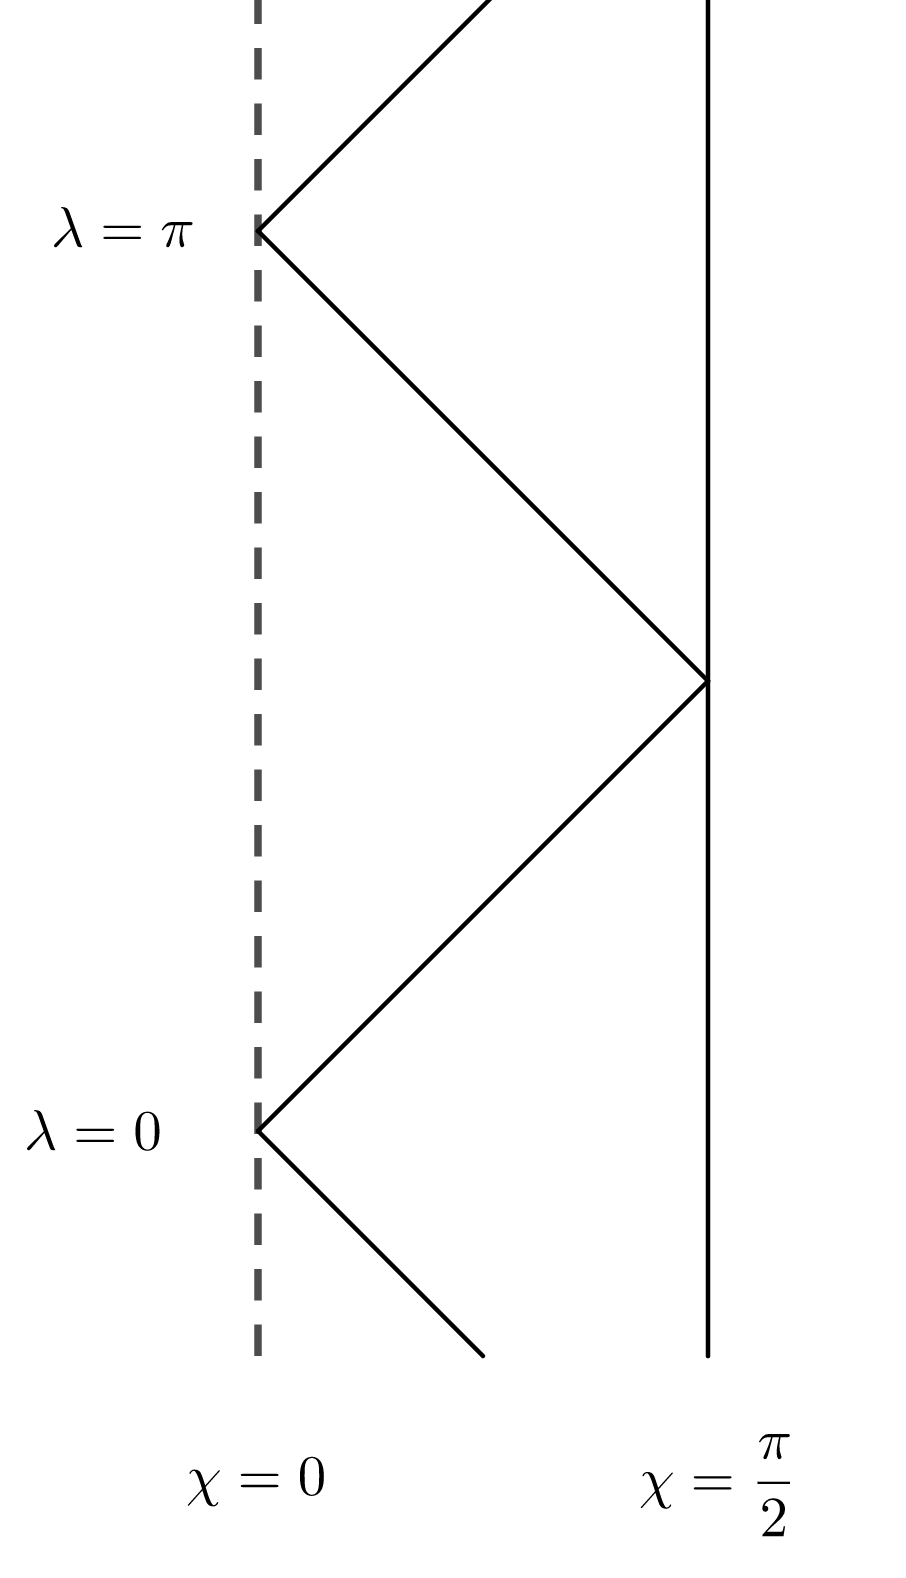
\includegraphics[width=0.35\textwidth]{../pics/AdS3_Pen.png}
%
\caption{Conformal diagram of anti-de Sitter space. We see that light rays can emerge at conformal infinity $\mathcal{J}$ at any $\lambda$, and subsequently terminate at $\mathcal{J}$ at a later $\lambda$. Thus, there are no \textbf{Cauchy surfaces} in $AdS_3$, and consequently we do not have well-posed initial value problems on the $AdS_3$ spacetime.}
%
\label{fig:penrose_ads}
%
\end{figure}
%
%
\noindent
%
Looking at the above conformal digram, we see a very interesting causal property of $AdS_3$, namely that conformal infinity $\mathcal{J}$ is a time-like hypersurface. As a consequence of this fact, $AdS_3$ is not globally hyperbolic, meaning that it has no \textbf{Cauchy surfaces}. This is because there exists null geodesics which both emerge and terminate at $\mathcal{J}$. Thus, we do not have well-posed initial value problems on the $AdS_3$ in terms of information specified on a Cauchy surface. Later in section 4.1, when we compute \textbf{Green's functions} on the BTZ spacetime, the fact that $AdS_3$ is not globally hyperbolic will force us to choose boundary condition for the scalar field at infinity. More details will follow in said section.

%%%%%%%%%%%%%%%%%%%%%%%%%%%%%%%%%%%%%%%%%%%%%%%%%%%%%%%%%%%%%%%%%%%%%%%%%%%%%%%%%%%%%%%%%%
%\subsubsection{Describtion in terms of SL(2, R)}
%Points in the ambient space can be represented by $2 \times 2$ real matrices. Let us for future convinience introduce the following basis on the space of $2 \times 2$ real matrices:
%%
%%
%\begin{equation}
%\gamma^0 = \frac{1}{l} \, \bigg( \begin{array}{cc}
%1 & 0 \\
%0 & 1
%\end{array} \bigg)
%\; , \;
%\gamma^1 = \frac{1}{l} \, \bigg( \begin{array}{cc}
%0 & 1 \\
%-1 & 0
%\end{array} \bigg)
%\; , \;
%\gamma^2 = \frac{1}{l} \, \bigg( \begin{array}{cc}
%1 & 0 \\
%0 & -1
%\end{array} \bigg)
%\; , \;
%\gamma^3 = \frac{1}{l} \, \bigg( \begin{array}{cc}
%0 & 1 \\
%1 & 0
%\end{array} \bigg)
%\end{equation}
%%
%%
%Where $l \in \mathbb{R}_+$. We can now represent a points in the ambient space by a matrix $\mathbf{X}$:
%%
%%
%\begin{equation}
%\mathbf{X} = x_a \, \gamma^a
%= \frac{1}{l} \, \bigg( \begin{array}{cc}
%x_0 + x_2 & x_1 + x_3 \\
%-x_1 + x_3 & x_0 - x_2
%\end{array} \bigg)
%\quad , \quad
%||x||^2
%= \eta^{ab}_{2,2} \, x_a \, x_b
%= -l^2 \, \det(\mathbf{X})
%\end{equation}
%%
%%
%Where $a \in \{ 0,1,2,3 \}$. From the above relations, we see that the norm preserving transformations on the abient space (\textit{elements of $SO(2,2)$}) can be reresented by elements of $\mathrm{SL}(2, \mathbb{R}) \times \mathrm{SL}(2, \mathbb{R}) / \mathbb{Z}_2$, acting on the $2 \times 2$ matrices in the following way:
%%
%%
%\begin{equation}
%\mathbf{X} \to  \rho_R \, \mathbf{X} \rho_L
%\quad , \quad
%(\rho_R, \rho_L) \in \mathrm{SL}(2, \mathbb{R}) \times \mathrm{SL}(2, \mathbb{R}) / \mathbb{Z}_2
%\end{equation}
%%
%%
%From the definition above, it is clear that the $\mathbb{Z}_2$ identification must be $(\rho_L, \rho_R) \sim (-\rho_L, -\rho_R)$. The constraint (\ref{anti-de sitter}) can now be expressed in terms of the $2 \times 2$ real matrices defined above:
%%
%%
%\begin{equation}
%\eta^{ab}_{2,2} \, x_a \, x_b
%= -l^2
%\quad \Rightarrow \quad
%\det(\mathbf{X}) = 1
%\end{equation}
%%
%%
%It is evident that the entire isometry group (\textit{apart from the reflections}) of $adS$ is the $SO(2,2)$ group.
%%%%%%%%%%%%%%%%%%%%%%%%%%%%%%%%%%%%%%%%%%%%%%%%%%%%%%%%%%%%%%%%%%%%%%%%%%%%%%%%%%%%%%%%%%%

\subsubsection{Constructing the BTZ spacetime}
As we have already mentioned previously, any solution to the vacuum Einstein Equatins in (2+1) must be locally isomorphic to $AdS_3$. Thus, the BTZ spacetime must also be locally isomorphic to $AdS_3$. However, there is no guarantee that the global structure of the BTZ spacetime should be related to that of $AdS_3$ in any simple way. Fortunately, it turns out that the global structures of BTZ and $AdS_3$ actually \textit{is} related in a simple way. This is most easilly seen by covering the hypersurface (\ref{anti-de sitter}) with a set of coordinates $(t, r, \phi)$, as defined in appendix B. It is easy to verify that the pull-back of the metric (\ref{ambient_metric}) onto the $AdS_3$ hypersurface, using the coordinates $(t, r, \phi)$, recovers the BTZ metric (\ref{btz_metric}) in each of the regions \textbf{I}, \textbf{II} and \textbf{III}, with $\Lambda = -\ell^{-2}$. In order for the $(t, r, \phi)$ coordinates to cover all of $AdS_3$, they must have the following ranges:
%
%
\begin{equation}
r \in (0, r_-) \cup (r_-, r_+) \cup (r_+, \infty)
\quad , \quad
\phi \in (-\infty, \infty)
\quad , \quad
t \in (-\infty, \infty)
\end{equation}
%
%
This is exactly the ranges of the  Schwarzschild-like coordinates on the BTZ spacetime, except that $\phi$ is here an uncompact coordinate. Thus, we arrive at the amazing fact that the BTZ spacetime can be constructed from $AdS$, by identifying points such that $\phi \sim \phi + 2 \pi$. This fact will greatly aid us in section 4.1, when we set out to find Green's functions on the BTZ spacetime.
